\section{Technical appendix}\label{sec:appendix}
\subsection{Terminology}\label{sec:terminology}

For clarity, we define some terms that have been used
throughout this proposal. We illustrate the terms in the context of the
reproducibility example in Section~\ref{sec:reproducibility-example}.

In particular, we imagine that we have a publication that contains
figure~\ref{fig:reproducibility-example-covid} as a result, and we want to
archive and make available \cite{ReproducibilityRepositoryExample2022} the
necessary information for others to reproduce that figure.

\begin{description}
\item[Repository] We refer to a \emph{repository} as a collection of files.

The \emph{purpose} of the repository in our context is to archive information to make
research results reproducible.

Such a repository could be a git repository (which could be hosted on GitHub,
Bitbucket, GitLab, or other services), but it could also just be a zip file of a
collection of files.

The repository could be made publicly available, for example through Zenodo,
Figshare, as an electronic supplementary to a publication, or through GitHub.

It is not unusual that a larger number of files might be
organised in subdirectories within the repository.

Our example repository\footnote{
  https://github.com/fangohr/reproducibility-repository-example/} \cite{ReproducibilityRepositoryExample2022} contains the following files:

\begin{description}
\item[\softwarename{README.md}]: an overview of the content of the repository
\item[\softwarename{figure1.ipynb}]: notebook that creates
  \softwarename{figure1.pdf} from
  the raw data. Could also be realised through a script or other executable
  program of some kind.
\item[\softwarename{requirements.txt}]: software specification
\item[\softwarename{time\_series\_covid19\_deaths\_global.csv}]: raw data
\end{description}

\item[Script] A machine-executable file (for example a Bash, Python, Perl
script, Makefile or similar). Such scripts can execute data processing commands,
and are often part of a repository to make the (automatic) reproduction of
results possible.

In our example, the necessary steps to create the figure from the raw data are
gathered in the notebook \texttt{figure1.ipynb}.

\item[Notebook] A Jupyter notebook. In short, an executable document that can
  combine text, code, and computation results. A Jupyter notebook can be used like a
  script. The notebook is explained in Section \fullref{sec:jupyter-notebook}.

\item[Software specification] The software specification depends on the software
  tools used. In our example, the \texttt{requirements.txt} file contains
\begin{verbatim}
pandas==1.3.4
matplotlib==3.4.3
\end{verbatim}
to indicate that we need the pandas and matplotlib package with the respective
versions 1.3.4 and 3.4.3.

\item[Software environment] All the software that needs to be available and
  installed to execute the scripts and (and if desired) Jupyter notebooks.

\item[Project Binder] The Project Binder is described in Section
\ref{seq:project-binder}. It is part of the Jupyter ecosystem of tools, and
allows to convert a repository with Jupyter notebooks into an browser-hosted
environment, in which the notebooks can be executed interactively (and thus
results can be reproduced).

\item[Binder tools] The Binder tools consist of \binderhub{}
  (Section~\ref{sec:binderhub}) and \repotodocker{} (see
  Section~\ref{sec:repo2docker}) .

\item[\repotodocker] \repotodocker{} is a tool that can automatically create a
\emph{software environment} (currently within a Docker container) in which the
notebooks and scripts of a repository can be executed
(Section~\ref{sec:repo2docker} and \ref{binder-how-does-it-work}).
\end{description}

\subsubsection{Project Jupyter}
\label{sec:project-jupyter}

% Figure has been moved into concept.tex. Label remains the same.
% \begin{figure}[htb]\centering
%   \includegraphics[width=0.9\textwidth]{use-cases-binder-logbook-solution.png}
%   \caption{A typical use case for Jupyter notebooks in research.
%             Image by Juliette Belin for the OpenDreamKit project, used under
%             CC-BY-SA.}\label{fig:use-cases-binder}
% \end{figure}

\paragraph{Relationship between the \TheProject{}project and the Jupyter ecosystem}

Some of the team member of the proposed SOURCE project have a track record as
developers and contributors to Project Jupyter and its associated
ecosystem, including Jupyter Notebook.

In opening this section, we'd like to state that the proposed work will improve
the reproducibility of research that uses notebooks, but that it is a key aspect
of the proposal to make the potential impact of the Binder tools for
reproducibility available to those researchers who have no desire or possibility
to use notebooks in their work.

In this section, we introduce key components of project Jupyter to help
contextualise the Binder project that is described subsequently, and the focus
of the proposed work.


% \TheProject has chosen to centre its efforts on the Jupyter software
% ecosystem, in particular Binder and repo2docker.
% Figure~\ref{fig:use-cases-binder} summarises a typical use
% case of Jupyter Notebook and Binder;
% both are described in more detail below.


\paragraph{Project Jupyter}

\emph{Project Jupyter} \cite{Jupyter}, which has grown increasingly popular in the scientific
computing community, has become the \emph{lingua franca} of interactive
computing in both academia and industry \cite{Perkel2018}. The main goal of Project Jupyter
is to provide a consistent set of tools to improve researchers'
workflows from the exploratory phase of the analysis to the communication
of the results \cite{Kluyver2016,Granger2021}.

Split in 2014 from the \emph{IPython Project} \cite{IPython}, Jupyter has grown rapidly in
popularity and adoption both in the industry and academia. We estimate the user
base of the Jupyter notebook to be in the millions \cite{jupyter-grant}. Users range from data
scientists to researchers, educators, and students from many fields,
including journalists and librarians. In 2017, the Jupyter
team was awarded the \emph{ACM Software System Award}, an annual award that
honors people or an organization \emph{"for developing a software system that had a
lasting influence"}. Prior recipients include \emph{Unix}, \emph{TCP/IP}, and
the \emph{World Wide Web} \cite{acm-award}.

A large number of discrete software components make up Project Jupyter.
While these interact with one another, many can be installed separately
to serve various use cases.

% For this proposal, we loosely divide the
% software involved into \emph{Jupyter core} developed under the guidance
% of the developers who started the project, and the broader \emph{Jupyter
% ecosystem} including software developed by third parties,
% which may interact or build upon core Jupyter components.

Some of the components and concepts important to \TheProject are detailed below.

\begin{figure}[ht]\centering
  \centering
  \includegraphics[width=0.9\textwidth]{spectrogram_smaller.png}
  \caption{A notebook document in the Jupyter Notebook interface.}\label{fig:notebook-screenshot}
\end{figure}

\paragraph{Jupyter Notebook}\label{sec:jupyter-notebook} The Jupyter Notebook is
the flagship application of Project Jupyter. 
It allows the creation of notebook documents, containing a mixture of text and
interactively executable code, along with rich output from running that code.
Figure \ref{fig:notebook-screenshot} shows an open notebook including graphs
from an audio processing example. Notebook documents are readily shareable,
providing a popular way to describe and illustrate computational methods and
tools. \TODO{We should update the notebook: (i) point to a github repo with it,
  and (ii) binder-enable it, and (iii) increase the pixel resolution of the
  screen shot. Madison?} \textbf{Jupyter Lab} is the new, modular, extensible
client application for Jupyter notebooks, but the document format, server, and
user model are the same.

\paragraph{JupyterHub}\label{sec:jupyterhub} JupyterHub is a multi-user extension of the Jupyter Notebook.
It runs on one or more notebook servers, for example at a research institution.
Users can log in to author and run notebooks through their web browser, without
needing to install any software on their own computer (because the research
software that is executed is located with the JupyterHub installation at the
research institution).

The communication between the notebook server (for example at the research
institution) and the client (for example the researcher with their laptop in the
home office) is based on the standard https protocol, and the connection is
efficient. The researcher - as the client of the connection to the JupyterHub -
only needs a web browser, and very modest hardware to be able to access
supercomputers or cloud resources remotely.

\TODO{Add an image with a schematic of JupyterHub here?}

Because of these characteristics, many research institutions host their own
JupyterHub service to provide access to large compute and data hosting
hardware~\cite{Fangohr2020}. JupyterHub installations are also seen as important
for EOSC, for example~\cite{panosc-jupyter-binder}. \TODO{Would be good to list
  one or two more EOSC projects / activities / EGI JupyterHub link}


% \medskip\noindent\emph{Jupyter ecosystem}\label{jupyter-ecosystem}
% 
% While Jupyter is a large, distributed, coordinated project,
% the wider community of Jupyter users develops a great deal of
% software with Jupyter integration,
% providing increased or domain-specific functionality,
% building on top of Jupyter, or integrating core Jupyter components in some aspect.
% We call this the \textbf{Jupyter ecosystem}.
% The broader Jupyter ecosystem includes many more projects than we will describe
% here, but a selection of projects which are relevant to
% \TheProject includes:
% 
% \begin{itemize}
%   \item \textbf{Binder} builds on JupyterHub to allow sharing executable
%   environments along with data files and a description of the software components
%   required to run the notebooks. When someone accesses a Binder repository,
%   the service builds the computational environment on demand, allowing them to
%   execute and modify a copy of the notebooks.
%   \textbf{repo2docker} \cite{repo2docker} and \textbf{BinderHub} \cite{binder} are components of the Binder
%   software. \TOWRITE{}{More here, as repo2docker is key}
% \end{itemize}

% \begin{figure}[ht]\centering
%   \includegraphics[width=0.5\textwidth]{ipywidgets_example.png}
%   \caption{An example of using two simple slider widgets to explore the
%   parameter space of a function. The \texttt{@interact} decorator creates
%   the widgets and connects them to the function.}
%   \label{fig:ipywidgets-example}
% \end{figure}

\paragraph{Jupyter notebook and reproducibility}

While Jupyter notebooks can make computational and data-driven research more effective
\cite{Perkel2018,Fangohr2020,Granger2021}, they also have great potential to push
Open and Reproducible Science forward \cite{Beg2021}. The notebook provides a complete
description of a computational and data science study (Step 1 in
figure~\ref{fig:use-cases-binder}), and the notebook can -- in principle -- be
turned into a publication, or can be used to provide the required computation
for a part of a publication, such as a figure (Step 2 in
figure~\ref{fig:use-cases-binder}). Once the researcher has specified what
software is required to execute the notebook (Step 3 in
figure~\ref{fig:use-cases-binder}), the study is completely reproducible by
anyone (Step 4 in figure~\ref{fig:use-cases-binder}).

In this way, the notebook \emph{enables reproducibility} of complex workflows
with minimal additional effort on the user side. This approach is used by a
substantial number of scientists for publications already (for example
\TODO{insert publications with reproducible repositories}): it is hard to prove
but it seems plausible that a significant fraction of the 30,000 sessions
triggered on MyBinder every day are used for reproducible repositories
(Section~\ref{sec:mybinder}).

% HF: this is a reference to the Joel Grus criticism. Not sure if we need it.
% The paper by Beg2021 addresses that in section 9.
(We note in passing that the use of Jupyter notebooks alone does not guarantee
reproducibility: it requires some training and/or experience to be able to specify a
computational environment and to capture in a machine readable way all required
computational steps.)

The Binder tools (Section~\ref{seq:project-binder}) were designed to execute
such notebooks in tailored computational environments which can be created
automatically and on demand (Step 4 in figure~\ref{fig:use-cases-binder}).

This fully-automatic creation of the correct software environment is an
essential aspect of reproducibility that is not widely addressed yet. This
project will address this need, improve the automatic software creation support
for notebook-driven computational research, and make the same improved automatic
software creation support accessible for uses cases without notebooks.

%%% Local Variables:
%%% mode: latex
%%% TeX-master: "proposal"
%%% End:

\subsubsection{Project Binder}\label{seq:project-binder}

The Binder Project \cite{binder} (\url{https://jupyter.org/binder}) is
a subproject of the Jupyter project. The Binder project is formally operating
within the Jupyter ecosystem, but not confined to be useful only for notebooks.

The key components of the Binder software are \repotodocker{}
(Section~\ref{sec:repo2docker}) and \binderhub{}. The \repotodocker{} tool
creates a software environment inside a Docker container from a software
specification in a repository. \binderhub{} starts a Jupyter notebook server
within this container from which the user can execute the notebooks from the
repository.

\emph{\mybinder{}} (see \ref{sec:mybinder}) is a service provided by the \emph{BinderHub
  federation} that collectively host a service running the Binder software
under the URL \url{https://mybinder.org}. This is the service we made use of in
our example in section~\ref{sec:reproducibility-example}.

The focus for this proposal is to improve \repotodocker{}. In particular,
\repotodocker{} solves the software environment challenge (see
Section~\ref{sec:reproducibility-concept}) in a generic way and is independent
from Jupyter notebooks.

\TODO{Add image that depicts this Jupyter/Binder relation ship}.

\paragraph{Basic functionality of Binder}
\label{binder-how-does-it-work}

The currently most common reproducibility use case -- with the current state of the Binder
tools -- is the one we introduced in
Section~\ref{sec:reproducibility-example}. We will use this to
describe the role of the individual components of Binder:


\begin{figure}
  \begin{minipage}[b]{0.67\textwidth}
    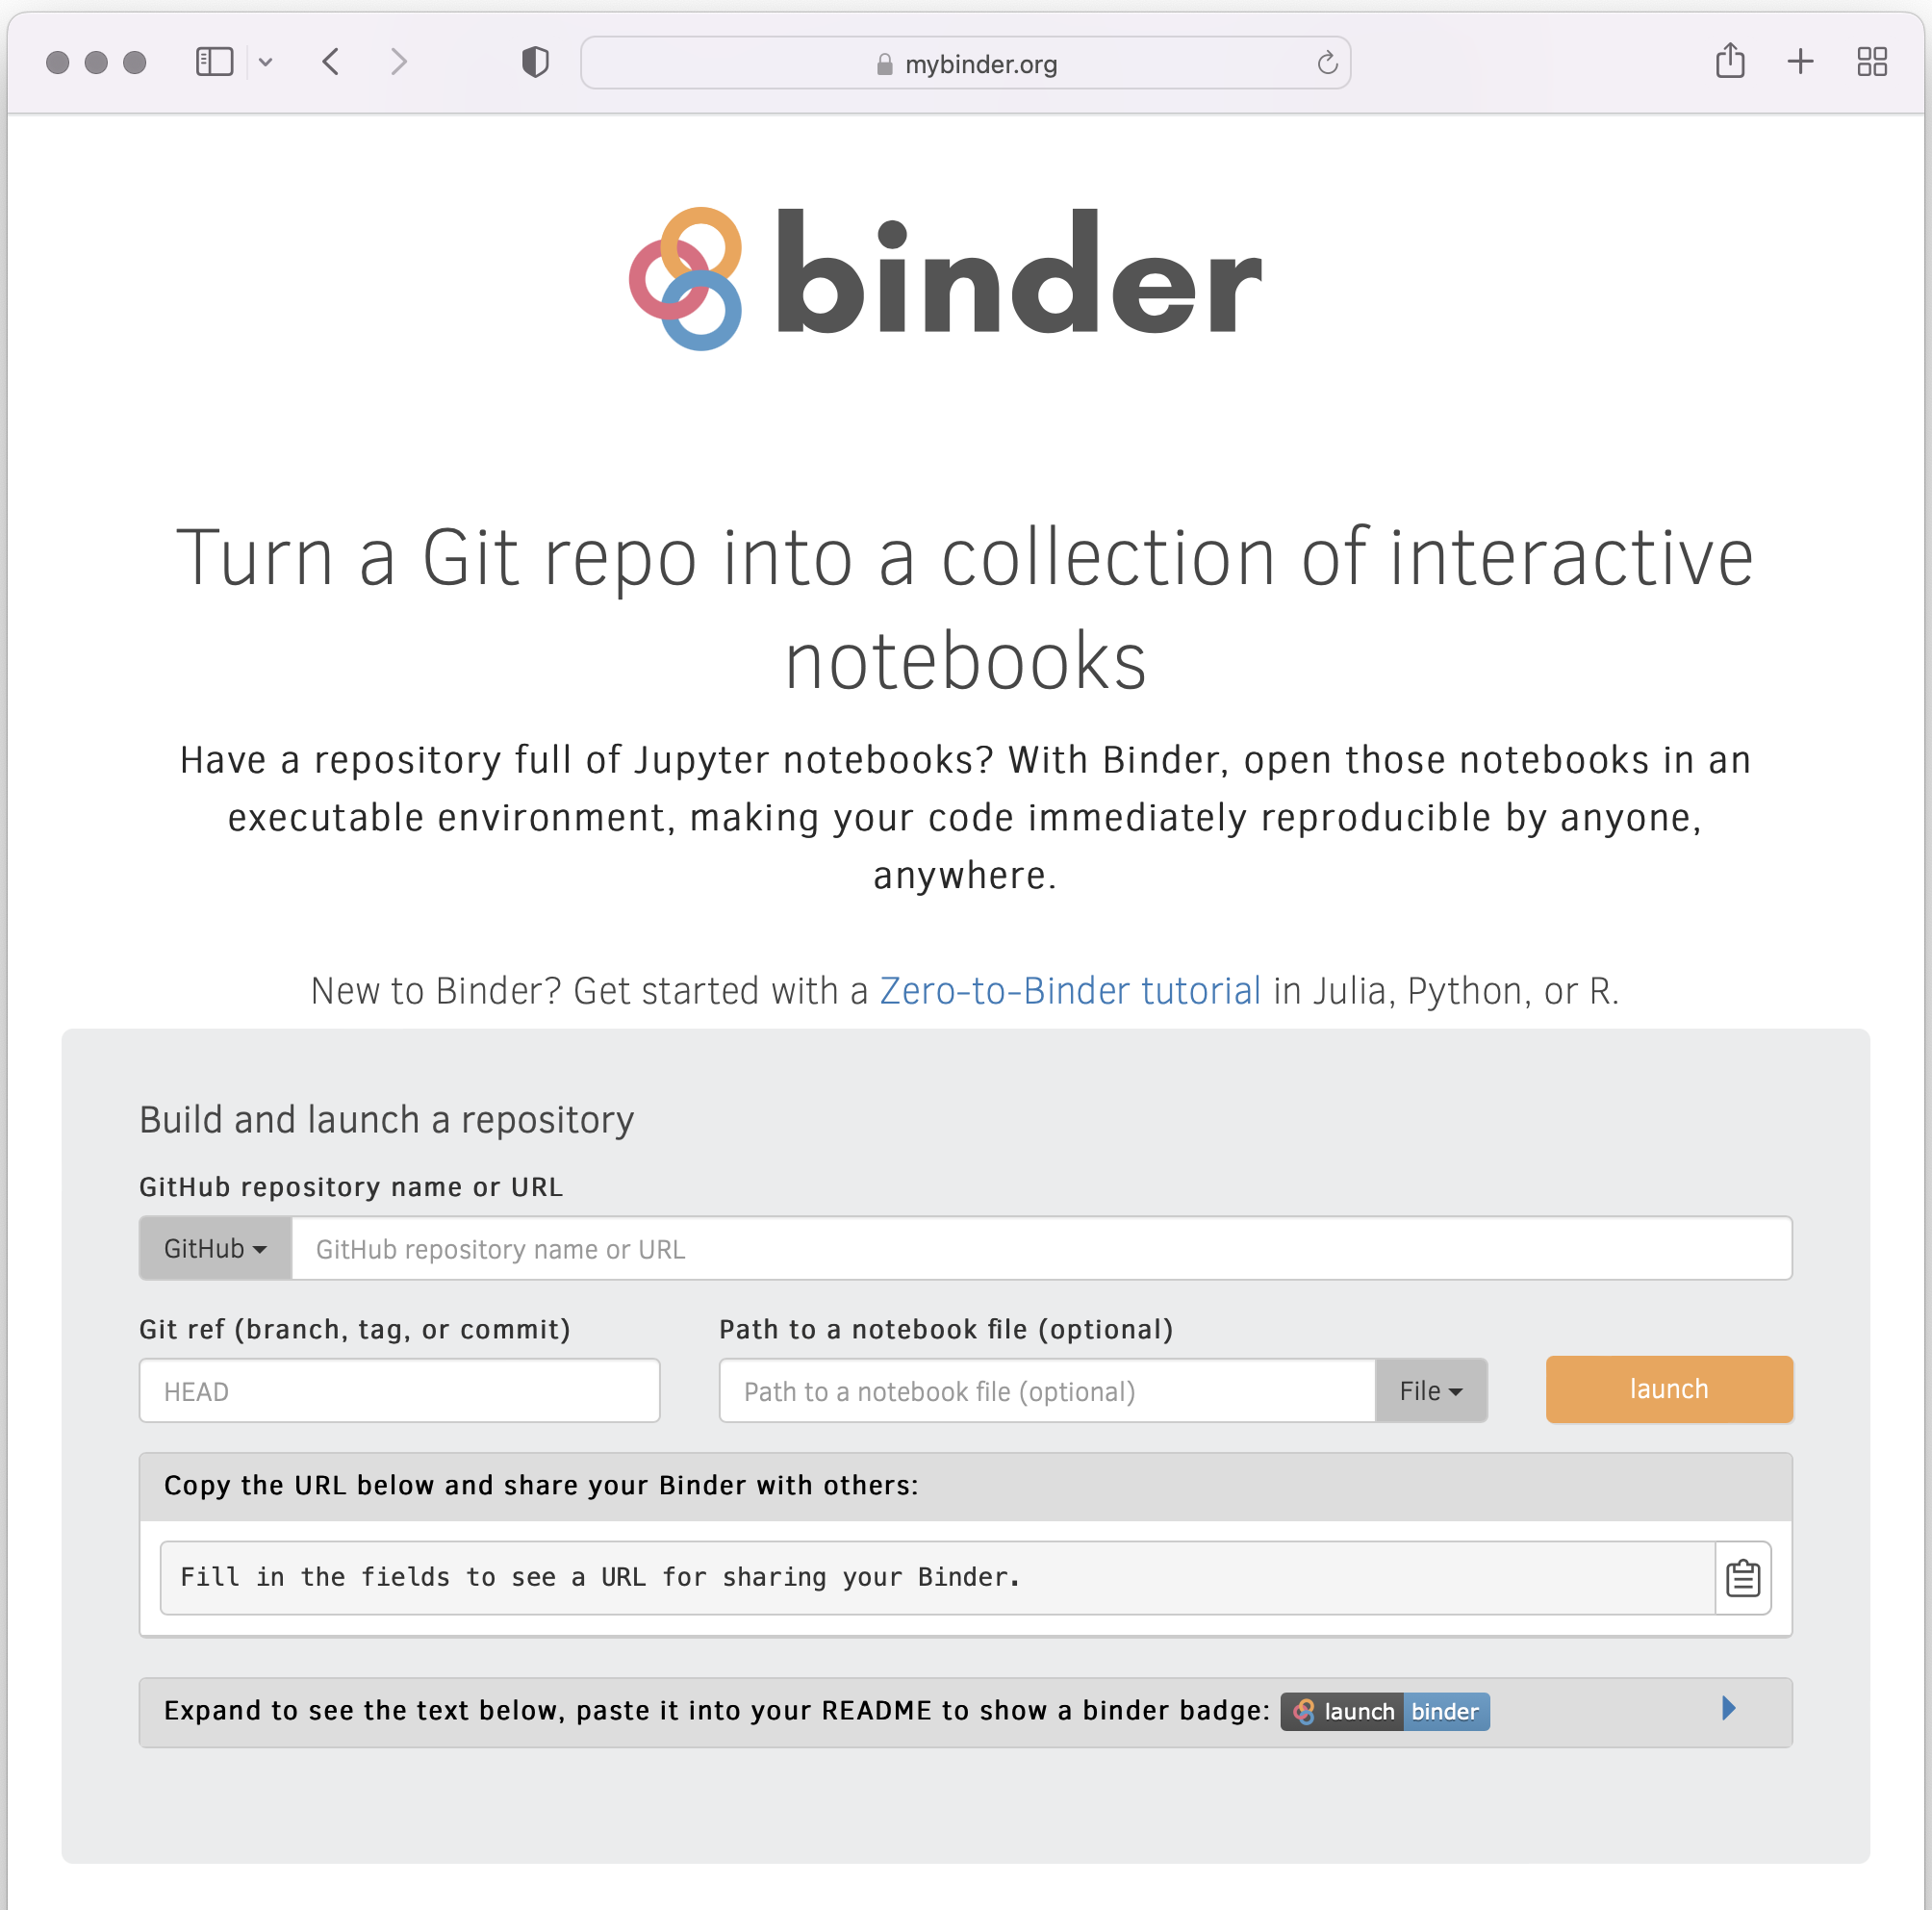
\includegraphics[width=1.0\textwidth]{images/mybinder.png}
  \end{minipage}\hfill
  \begin{minipage}[b]{0.3\textwidth}
    \caption{Home page of the \mybinder{} service.}  \label{fig:mybinder-homepage}
  \end{minipage}
\end{figure}


\begin{compactitem}
\item The \mybinder{} service is called with a URL that encodes the location of the data
  repository\footnote{For example the 
    {\url{https://mybinder.org/v2/gh/fangohr/reproducibility-repository-example/HEAD?labpath=figure1.ipynb}}
    refers to the GitHub repository ``reproducibility-repository-example'' of the
    github user ``fangohr'', asking to open the ``figure1.ipynb'' file.}

  Alternatively, there is form (see Figure~\ref{fig:mybinder-homepage})
  which users can complete with repository details
  to start the build of the corresponding environment, or to obtain the URL to
  re-use that configuration later, or share it with others.
\item From the \mybinder{} entry point, the request is forwarded to one
  \binderhub{} service of one of the organisations in the BinderHub federation
  that has available compute resources.
\item The \binderhub{} software running at the chosen location, will ask
  \repotodocker{} to create a Docker container in which the notebooks from the repository can be executed.
\item \repotodocker{} searches the repository for specifications of software requirements (see \ref{repo2docker-supported-software-specifications}).
\item \repotodocker{} composes a Dockerfile that contains all the commands
  necessary to install software.
\item \repotodocker{} builds the Docker image based on the Dockerfile.
\item \binderhub{} takes the Docker image and asks Kubernetes to start 
  a container based on this image.
\item The notebook server is started in this Docker container.
\item \binderhub{} forwards the user who requested this virtual environment to
  the URL at which the repository (or a particular notebook) can be explored
  from within the Jupyter notebook (which runs in the container).
\end{compactitem}

\paragraph{The repo2docker software tool.}\label{sec:repo2docker}

\repotodocker{} is a tool to fetch a remote repository and build a software
environment for this repository. Currently, \repotodocker{} can retrieve
repositories from the following services and formats: GitHub, Gist, Git, GitLab,
Zenodo, Hydroshare, Figshare, Dataverse.

For the automatic building of reproducible computational environments,
\repotodocker{} understands commonly used conventions for environment specifications and
community standard tools such as Docker, conda, mamba, and pip. See
Section~\ref{repo2docker-supported-software-specifications} below for a full list of
currently supported software specifications.

\paragraph{Supported software specification formats}
\label{repo2docker-supported-software-specifications}
The \repotodocker{} tool currently supports the following software specification
formats to build Docker images:
% source:
% https://repo2docker.readthedocs.io/en/latest/config_files.html#config-files
% 9 April 2022
\begin{compactitem}
\item \softwarename{requirements.txt}, \softwarename{setup.py},
  \softwarename{Pipfile}, \softwarename{Pipfile.lock}: to specify Python
  packages and environments
\item \softwarename{Project.toml}, \softwarename{JuliaProject.toml} and (legacy)
  \softwarename{REQUIRE}: to
  specify Julia version and packages
\item \softwarename{install.R}, \softwarename{DESCRIPTION}: to install R
  libraries, or install the repository as R package
\item \softwarename{apt.get}: to install Debian packages. The Docker container
  is currently based on Ubuntu, which uses the Debian package management tool \softwarename{apt}.
\item \softwarename{environment.yml}: to specify conda or mamba packages and
  environments
\item \softwarename{default.nix}: to use the nix package manager for software provision
\item \softwarename{Dockerfile}: providing a Dockerfile enables users to define
  virtually arbitrary environments, for example based on software from the
  repositories of Linux distributions.
\end{compactitem}

\paragraph{BinderHub}\label{sec:binderhub}
BinderHub is software for hosting a web service built on \repotodocker{} and
JupyterHub where individuals can share reproducible environments for
immediate and free interaction by readers in their browser.


\paragraph{The \mybinder{} service}\label{sec:mybinder}

\emph{\mybinder{}} is a service run by the \emph{BinderHub
  federation}\footnote{\url{https://mybinder.readthedocs.io/en/latest/about/federation.html}}
of organisations. Collectively, they host a service running the BinderHub software
which can be reached from \url{https://mybinder.org}.

The service is actively used with approximately 200,000 sessions being
requested and delivered by the \mybinder{} service every week in 2021. The number
of sessions is growing from approximately 10,000 per day in November 2018
(beginning of the available records) to about 30,000 per day in 2022. We have
identified 60,000 unique repositories published in the last few years which have
used the \mybinder{} service. The data is available~\cite{mybinder-archive}.

Examples of reproducible repositories that make use of the \mybinder service
include reproducible research repositories
\cite{GitHubRepoExampleAlbert2016,Beg2021}, interactive textbooks
\cite{Fangohr2022,Zeller2022} and citizen science and outreach activities
\cite{ligo-open-science,OSCOVIDA2022}.

This \TheProject{} project will not provide or operate a BinderHub service (such as the global
``\url{https://mybinder.org}'' instance). The improvements achieved, however, will immediately
be made available to all operators of BinderHubs, including \mybinder{}.


% \subsubsection{Binder for reproducibility}\label{sec:binder-for-reproducibility}
% \TOWRITE{}{Hmm -- perhaps we don't need this section, as we explain in the
%   Methodology section what we want to do with Binder?}




%%% Local Variables:
%%% mode: latex
%%% TeX-master: "proposal"
%%% End:



% Not relevant here. Should remove that file later.
% % This section is probably not needed for SOURCE.

\medskip
\noindent\textbf{Jupyter as a basis for web services}\\
Because the Jupyter notebook is a web-based application, it can be
deployed at computational facilities or in the cloud, and can function
as the basis for services exposing computational resources of all
kinds to researchers and the public.  Because Jupyter is
\textbf{interactive}, it enables making scientific results and
communications more interactive than static publications.  The
audience can follow their own initiative and ask their own questions
of published data without needing support from the publishing author,
greatly facilitating the \textbf{practicality of Open Science}.

\medskip
\noindent\textbf{Jupyter is generic}\\
\TheProject chose Jupyter because it is
Generic.  Jupyter makes no domain-specific or even language-specific
assumptions.  Any application where mixing description, code, and
results is valuable can make use of Jupyter.  This broad applicability
makes investment in the Jupyter ecosystem extremely effective, because
improvements to Jupyter can serve many communities simultaneously.

Jupyter is built from a collection of standard protocols and file
formats.  Jupyter is not just a single, monolithic piece of
software, but a description of how such software can be built.  The
result is the ability for a variety of communities and applications to
use components of Jupyter for their purposes, and/or reimplement pieces to
meet their needs.
%
For example:
\begin{enumerate}
\item The notebook file format is a well-specified JSON document,
  which can be interpreted by many systems.  This has facilitated the
  development of different services providing rendering of notebooks, e.g. the code
  hosting website GitHub, which renders notebooks for easy viewing by
  anyone, without Jupyter software.
\item The Jupyter protocol describes how execution is performed, which
  has enabled the development of over one hundred kernel
  implementations in dozens of languages\footnote{\url{https://github.com/jupyter/jupyter/wiki/Jupyter-kernels}}.
\item Output in the Jupyter protocol uses web-standard MIME types,
  enabling any possible format to be an output in a Jupyter notebook.
\item The JupyterLab extension system provides a system for building
  applications from Jupyter components and others.
\item The Jupyter Widgets provide a system for customising and
  extending interactivity in Jupyter-based environments.
\end{enumerate}

The popularity of Jupyter, with millions of users and hundreds of open
source contributors, is an indicator of the value and impact of this approach.

\medskip
\noindent\textbf{Improvement to the Jupyter ecosystem}\\
The benefits of focusing our work on a mature system like Jupyter include:

\begin{itemize}
\item vibrant community ensures health and sustainability,
\item large existing user base maximises impact of contributions,
\item mature software ecosystem maintains quality software through
  industry standards such as version control, tests, continuous
  integration, stable release cycles, roadmaps, and user support.
\end{itemize}

The Jupyter community aims to be inclusive, and \TheProject fully
embraces and supports that approach.  Jupyter is inclusive across a number of axes.
By being applicable across numerous domains, Jupyter and \TheProject
encourage participation from individuals of various interests and
backgrounds, and has taken action to improve diversity in the project
by participating in ``Outreachy,'' a program of paid internships for
individuals from groups that face under-representation, systemic bias,
or discrimination.  Jupyter has also operated workshops focused on
training contributors from under-represented groups.  In being free,
public, open source software, Jupyter and \TheProject are accessible
to as many individuals as possible, and invites users and contributors
beyond origin, nationality, beliefs, orientation.  One area where
Jupyter has lacked in this regard is in the User Interface
accessibility, and we will help improve this in
% \taskref{core}{accessibility}
.  Additionally, the project will
focus some of its workshops in
% \taskref{education}{workshops}
on
under-represented communities.


\begin{figure}[ht!]\centering
  \includegraphics[width=0.6\textwidth]{images/notebook_components.png}
  \caption{The architecture of the Jupyter notebook, kernels, and tools
        which operate on notebook files}
  \label{fig:notebook-architecture}
\end{figure}


